\documentclass[11pt,a4paper]{article}

% ── Packages ──────────────────────────────────────────────────────────────────
\usepackage[utf8]{inputenc}
\usepackage[T1]{fontenc}
\usepackage{lmodern}
\usepackage[margin=2.5cm]{geometry}
\usepackage{graphicx}
\usepackage{amsmath,amssymb}
\usepackage{booktabs}
\usepackage{array}
\usepackage{multirow}
\usepackage{enumitem}
\usepackage{float}
\usepackage{caption}
\usepackage{subcaption}
\usepackage{hyperref}
\usepackage{xcolor}
\usepackage{listings}
\usepackage{algorithm}
\usepackage{algpseudocode}
\usepackage{tikz}
\usetikzlibrary{shapes.geometric, arrows.meta, positioning, fit, calc}
\usepackage{fancyhdr}
\usepackage{titlesec}
\usepackage[backend=biber,style=ieee]{biblatex}

% ── Colors ────────────────────────────────────────────────────────────────────
\definecolor{codeblue}{HTML}{2563EB}
\definecolor{codegray}{HTML}{6B7280}
\definecolor{codebg}{HTML}{F9FAFB}
\definecolor{linkcolor}{HTML}{1D4ED8}

% ── Hyperref ──────────────────────────────────────────────────────────────────
\hypersetup{
  colorlinks=true,
  linkcolor=linkcolor,
  citecolor=linkcolor,
  urlcolor=linkcolor,
  bookmarksnumbered=true,
}

% ── Listings ──────────────────────────────────────────────────────────────────
\lstset{
  backgroundcolor=\color{codebg},
  basicstyle=\ttfamily\small,
  keywordstyle=\color{codeblue}\bfseries,
  commentstyle=\color{codegray}\itshape,
  breaklines=true,
  frame=single,
  rulecolor=\color{codegray!30},
  numbers=left,
  numberstyle=\tiny\color{codegray},
  xleftmargin=2em,
  framexleftmargin=1.5em,
}

% ── Header / Footer ──────────────────────────────────────────────────────────
\pagestyle{fancy}
\fancyhf{}
\fancyhead[L]{\small\textsc{MathSnap-AI}}
\fancyhead[R]{\small\thepage}
\renewcommand{\headrulewidth}{0.4pt}
\fancypagestyle{plain}{\fancyhf{}\fancyfoot[C]{\small\thepage}\renewcommand{\headrulewidth}{0pt}}

% ── Title ─────────────────────────────────────────────────────────────────────
\title{%
  \vspace{-1cm}
  \textbf{MathSnap-AI}\\[0.3em]
  \large Compact Handwritten Mathematical Expression Recognition\\
  with Coverage-Aware Attention Refinement
}
\author{MathSnap-AI Project}
\date{March 2026}

% ══════════════════════════════════════════════════════════════════════════════
\begin{document}

\maketitle
\thispagestyle{plain}

% ── Abstract ──────────────────────────────────────────────────────────────────
\begin{abstract}
\noindent
MathSnap-AI is an end-to-end system for Handwritten Mathematical Expression Recognition (HMER) that converts photographs of handwritten mathematics into \LaTeX{} markup. The system is built on \textbf{Mini-CoMER}, a compact encoder--decoder neural network with 6.39\,M parameters---a 68\% reduction from the original CoMER architecture. Mini-CoMER pairs a DenseNet-based feature extractor with a Transformer decoder augmented by an Attention Refinement Module (ARM) that prevents redundant spatial attention. Trained on the CROHME dataset, the model achieves an expression recognition rate (ExpRate) of 47.12\% while maintaining real-time inference capability on consumer-grade GPUs. The full system comprises a FastAPI backend deployed on Hugging Face Spaces and a React frontend hosted on Vercel.
\end{abstract}

\vspace{0.5em}
\noindent\textbf{Keywords:} handwritten math recognition, encoder--decoder, attention refinement, DenseNet, Transformer, \LaTeX{} generation

\tableofcontents
\newpage

% ══════════════════════════════════════════════════════════════════════════════
\section{Introduction}
\label{sec:intro}

Handwritten Mathematical Expression Recognition (HMER) is the task of converting an image of a handwritten mathematical expression into a structured representation such as \LaTeX{}. Unlike standard OCR, HMER must capture two-dimensional spatial relationships---superscripts, subscripts, fractions, and nested structures---making it substantially more challenging.

MathSnap-AI addresses this problem with three objectives:

\begin{enumerate}[nosep]
  \item \textbf{Compactness.} Reduce model size to enable deployment on resource-constrained hardware without sacrificing recognition quality.
  \item \textbf{Coverage awareness.} Prevent the decoder from repeatedly attending to dominant symbols while ignoring others, a common failure mode in attention-based sequence generation.
  \item \textbf{Deployability.} Provide a complete, production-ready system with a web frontend, a REST API, and automated deployment.
\end{enumerate}

The resulting model, \textbf{Mini-CoMER}, contains 6.39\,M parameters (68\% fewer than the original CoMER) and runs inference in real time on a single consumer GPU.

% ══════════════════════════════════════════════════════════════════════════════
\section{Related Work}
\label{sec:related}

\textbf{Encoder--decoder approaches.} Early HMER systems used CNN encoders paired with RNN decoders with attention. WAP~introduced a coverage-based attention mechanism to address the under-attention problem. BTTR~replaced the RNN decoder with a bidirectional Transformer, improving parallelism during training.

\textbf{CoMER.} The Coverage-augmented Multi-head attention Enhanced Recognizer (CoMER) integrated an Attention Refinement Module (ARM) into multi-head cross-attention layers, explicitly tracking cumulative attention coverage. While effective, CoMER's ${\sim}$20\,M parameters made deployment on edge devices impractical.

\textbf{Model compression for HMER.} Prior work has explored knowledge distillation and channel pruning for optical character recognition, but few studies target HMER-specific architectures. Mini-CoMER takes a direct approach: narrowing the DenseNet growth rate and reducing decoder depth while retaining the ARM mechanism that is critical for expression-level accuracy.

% ══════════════════════════════════════════════════════════════════════════════
\section{Dataset}
\label{sec:dataset}

\subsection{CROHME}

The Competition on Recognition of Online Handwritten Mathematical Expressions (CROHME) dataset is the standard benchmark for HMER. MathSnap-AI uses the merged CROHME 2014/2016/2019 splits:

\begin{table}[H]
\centering
\caption{CROHME dataset split distribution.}
\label{tab:dataset}
\begin{tabular}{lrr}
\toprule
\textbf{Split} & \textbf{Samples} & \textbf{Proportion} \\
\midrule
Train      & 21{,}855 & 80.7\% \\
Validation &  1{,}702 &  6.3\% \\
Test       &  3{,}499 & 12.9\% \\
\midrule
\textbf{Total} & \textbf{27{,}056} & \textbf{100\%} \\
\bottomrule
\end{tabular}
\end{table}

\subsection{Vocabulary}

The vocabulary contains 114 tokens: 4 special tokens (\texttt{<PAD>}, \texttt{<SOS>}, \texttt{<EOS>}, \texttt{<UNK>}) and 110 \LaTeX{} tokens spanning digits, Latin and Greek letters, operators, functions, structural commands, delimiters, and mathematical symbols.

\begin{table}[H]
\centering
\caption{Vocabulary composition.}
\label{tab:vocab}
\begin{tabular}{ll}
\toprule
\textbf{Category} & \textbf{Examples} \\
\midrule
Special (4)    & \texttt{<PAD>}, \texttt{<SOS>}, \texttt{<EOS>}, \texttt{<UNK>} \\
Digits (10)    & \texttt{0}--\texttt{9} \\
Letters (37)   & \texttt{a}--\texttt{z}, \texttt{A}, \texttt{B}, \texttt{C}, \ldots \\
Greek (10)     & \texttt{\textbackslash alpha}, \texttt{\textbackslash beta}, \texttt{\textbackslash gamma}, \texttt{\textbackslash theta}, \texttt{\textbackslash pi}, \ldots \\
Operators (17) & \texttt{+}, \texttt{-}, \texttt{=}, \texttt{\textbackslash times}, \texttt{\textbackslash leq}, \texttt{\textbackslash geq}, \ldots \\
Functions (5)  & \texttt{\textbackslash sin}, \texttt{\textbackslash cos}, \texttt{\textbackslash tan}, \texttt{\textbackslash log}, \texttt{\textbackslash lim} \\
Structural (8) & \texttt{\textbackslash frac}, \texttt{\textbackslash sqrt}, \texttt{\^{}}, \texttt{\_}, \texttt{\{}, \texttt{\}} \\
Delimiters (5) & \texttt{(}, \texttt{)}, \texttt{[}, \texttt{]}, \texttt{|} \\
Symbols (18)   & \texttt{\textbackslash infty}, \texttt{\textbackslash sum}, \texttt{\textbackslash int}, \texttt{\textbackslash forall}, \texttt{\textbackslash exists}, \ldots \\
\bottomrule
\end{tabular}
\end{table}

\subsection{Sequence Length Distribution}

Target sequences have a mean length of ${\sim}12$ tokens (median ${\sim}10$), with 95\% of samples below 30 tokens and a hard maximum of 200 tokens.

% ══════════════════════════════════════════════════════════════════════════════
\section{Model Architecture}
\label{sec:architecture}

Mini-CoMER follows an encoder--decoder design with three main components: a DenseNet encoder, a Transformer decoder, and an Attention Refinement Module (ARM).

\subsection{Architecture Overview}

\begin{figure}[H]
\centering
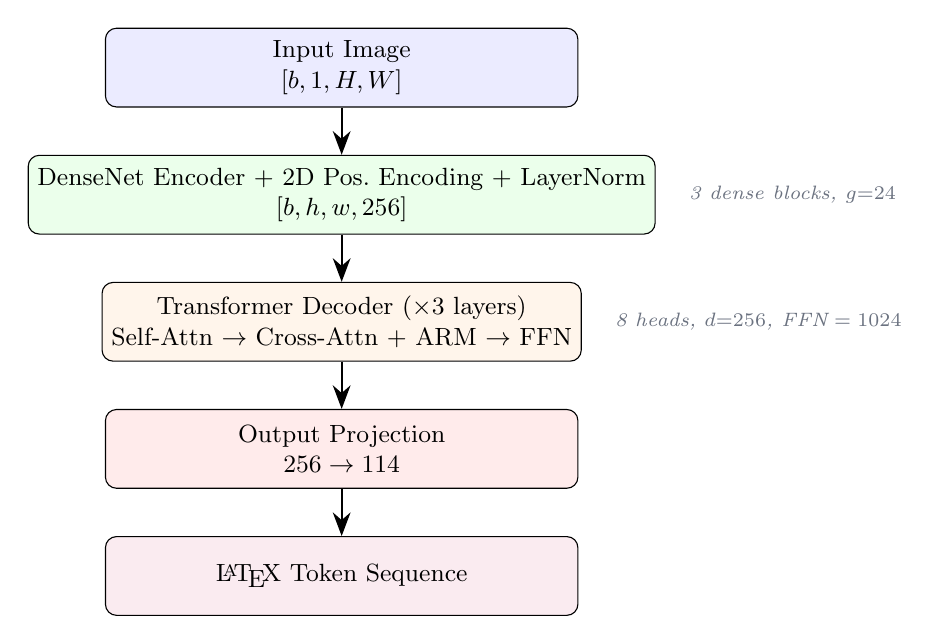
\begin{tikzpicture}[
  block/.style={draw, rounded corners, minimum width=6cm, minimum height=1cm, align=center, font=\small},
  arrow/.style={-{Stealth[length=3mm]}, thick},
  note/.style={font=\scriptsize\itshape, text=codegray},
]
  \node[block, fill=blue!8] (input) {Input Image\\$[b, 1, H, W]$};
  \node[block, fill=green!8, below=0.6cm of input] (encoder) {DenseNet Encoder + 2D Pos.\ Encoding + LayerNorm\\$[b, h, w, 256]$};
  \node[block, fill=orange!8, below=0.6cm of encoder] (decoder) {Transformer Decoder ($\times 3$ layers)\\Self-Attn $\to$ Cross-Attn + ARM $\to$ FFN};
  \node[block, fill=red!8, below=0.6cm of decoder] (proj) {Output Projection\\$256 \to 114$};
  \node[block, fill=purple!8, below=0.6cm of proj] (output) {\LaTeX{} Token Sequence};

  \draw[arrow] (input) -- (encoder);
  \draw[arrow] (encoder) -- (decoder);
  \draw[arrow] (decoder) -- (proj);
  \draw[arrow] (proj) -- (output);

  \node[note, right=0.3cm of encoder] {3 dense blocks, $g{=}24$};
  \node[note, right=0.3cm of decoder] {8 heads, $d{=}256$, FFN${}=1024$};
\end{tikzpicture}
\caption{Mini-CoMER architecture overview.}
\label{fig:architecture}
\end{figure}

\subsection{DenseNet Encoder}
\label{sec:encoder}

The encoder extracts spatial features from a grayscale input image using a DenseNet-B backbone with three dense blocks.

\begin{table}[H]
\centering
\caption{Encoder layer configuration.}
\label{tab:encoder}
\begin{tabular}{lll}
\toprule
\textbf{Stage} & \textbf{Operation} & \textbf{Output Shape} \\
\midrule
Input         & ---                                          & $[b, 1, H, W]$ \\
Initial conv  & $\text{Conv}(1{\to}48,\; 7{\times}7,\; s{=}2)$ + BN + ReLU & $[b, 48, H/2, W/2]$ \\
Max pool      & $2{\times}2,\; s{=}2$                        & $[b, 48, H/4, W/4]$ \\
Dense Block 1 & $16 \times \text{Bottleneck}(g{=}24)$        & $[b, 432, H/4, W/4]$ \\
Transition 1  & $\text{Conv}(1{\times}1,\; r{=}0.5)$ + AvgPool   & $[b, 216, H/8, W/8]$ \\
Dense Block 2 & $16 \times \text{Bottleneck}(g{=}24)$        & $[b, 600, H/8, W/8]$ \\
Transition 2  & $\text{Conv}(1{\times}1,\; r{=}0.5)$ + AvgPool   & $[b, 300, H/16, W/16]$ \\
Dense Block 3 & $16 \times \text{Bottleneck}(g{=}24)$        & $[b, 684, H/16, W/16]$ \\
Projection    & $\text{Conv}(684{\to}256,\; 1{\times}1)$     & $[b, 256, h, w]$ \\
Pos.\ encoding & 2D sinusoidal                               & $[b, h, w, 256]$ \\
LayerNorm     & ---                                          & $[b, h, w, 256]$ \\
\bottomrule
\end{tabular}
\end{table}

Each bottleneck layer consists of a $1{\times}1$ convolution expanding to $4g = 96$ channels followed by a $3{\times}3$ convolution producing $g = 24$ new feature channels. Dense connections concatenate the output of every layer to all subsequent layers within a block.

\subsubsection{2D Positional Encoding}

Standard Transformer positional encodings are one-dimensional. Since HMER requires awareness of both horizontal and vertical position (e.g., superscripts vs.\ subscripts), the encoder applies a 2D sinusoidal encoding:

\begin{equation}
\text{PE}_{(y,x,2i)} = \sin\!\left(\frac{y}{T^{2i/d}}\right), \qquad
\text{PE}_{(y,x,2i+1)} = \cos\!\left(\frac{y}{T^{2i/d}}\right)
\label{eq:posenc2d}
\end{equation}

where $T = 10{,}000$ is the temperature, $d = 256$ is the model dimension, and analogous terms are computed for the $x$ coordinate. Positions are derived from cumulative masks to handle variable-size images.

\subsection{Transformer Decoder}
\label{sec:decoder}

The decoder autoregressively generates \LaTeX{} tokens conditioned on the encoder features. It consists of a word embedding layer, 1D positional encoding, three Transformer decoder layers, and a linear output projection.

\begin{table}[H]
\centering
\caption{Decoder hyperparameters.}
\label{tab:decoder}
\begin{tabular}{lr}
\toprule
\textbf{Parameter} & \textbf{Value} \\
\midrule
Number of layers         & 3 \\
Attention heads          & 8 \\
Model dimension ($d$)    & 256 \\
Head dimension           & 32 \\
FFN inner dimension      & 1{,}024 \\
Dropout                  & 0.3 \\
Max sequence length      & 200 \\
Vocabulary size          & 114 \\
\bottomrule
\end{tabular}
\end{table}

Each decoder layer performs three sub-operations with residual connections and layer normalization:

\begin{enumerate}[nosep]
  \item \textbf{Causal self-attention} over the target sequence, preventing tokens from attending to future positions.
  \item \textbf{Cross-attention} to the encoder feature map, binding each output token to spatial image regions. The ARM (Section~\ref{sec:arm}) intervenes here.
  \item \textbf{Position-wise feed-forward network} ($256 \to 1024 \to 256$) with ReLU activation.
\end{enumerate}

\subsection{Attention Refinement Module (ARM)}
\label{sec:arm}

The ARM addresses the \emph{coverage problem}: without explicit tracking, the decoder tends to repeatedly attend to visually salient symbols while ignoring less prominent ones, causing missed or duplicated tokens.

\subsubsection{Mechanism}

Let $\alpha_t \in \mathbb{R}^{n_h \times S}$ denote the cross-attention weights at decoding step $t$ across $n_h = 8$ heads over $S = h \times w$ spatial positions. The ARM computes a coverage bias $\beta_t$ as follows:

\begin{align}
C_t &= \sum_{k=1}^{t-1} \alpha_k \label{eq:coverage} \\
\hat{C}_t &= \text{Conv}_{5 \times 5}\!\left(\text{reshape}(C_t)\right) \label{eq:conv} \\
\beta_t &= \text{MaskBN}\!\left(\text{Conv}_{1 \times 1}\!\left(\text{ReLU}(\hat{C}_t)\right)\right) \label{eq:bias}
\end{align}

The coverage bias $\beta_t$ is subtracted from the cross-attention logits before softmax, discouraging re-attention to already-covered regions.

\subsubsection{Configuration}

\begin{table}[H]
\centering
\caption{ARM hyperparameters.}
\label{tab:arm}
\begin{tabular}{lr}
\toprule
\textbf{Parameter} & \textbf{Value} \\
\midrule
Intermediate channels ($d_c$)  & 32 \\
Coverage kernel size           & $5 \times 5$ \\
Activation                     & ReLU \\
Post-normalization             & Masked BatchNorm \\
Cross-coverage                 & Enabled \\
Self-coverage                  & Enabled \\
\bottomrule
\end{tabular}
\end{table}

Masked BatchNorm applies normalization only over valid (non-padded) spatial positions, preventing padding artifacts from corrupting batch statistics.

\subsection{Parameter Budget}

\begin{table}[H]
\centering
\caption{Parameter breakdown: Mini-CoMER vs.\ original CoMER.}
\label{tab:params}
\begin{tabular}{lrr}
\toprule
\textbf{Component} & \textbf{Mini-CoMER} & \textbf{CoMER} \\
\midrule
DenseNet Encoder   & ${\sim}4.2$\,M & ${\sim}13$\,M \\
Transformer Decoder & ${\sim}2.1$\,M & ${\sim}6.5$\,M \\
ARM                & ${\sim}62$\,K  & ${\sim}170$\,K \\
\midrule
\textbf{Total}     & \textbf{6.39\,M} & \textbf{${\sim}$20\,M} \\
\bottomrule
\end{tabular}
\end{table}

The 68\% reduction is achieved by narrowing the DenseNet growth rate from 48 to 24, reducing decoder layers from 6 to 3, and lowering the FFN dimension from 2048 to 1024.

% ══════════════════════════════════════════════════════════════════════════════
\section{Preprocessing}
\label{sec:preprocessing}

Input images undergo a deterministic preprocessing pipeline before inference:

\begin{enumerate}[nosep]
  \item \textbf{Grayscale conversion.} The image is converted to a single-channel representation.
  \item \textbf{Otsu binarization.} An automatic threshold separates foreground (ink) from background, removing noise and uneven lighting.
  \item \textbf{Background detection.} Border pixels are sampled; if the majority are white ($> 128$), the image is inverted to ensure dark-on-light convention.
  \item \textbf{Aspect-ratio-preserving resize.} The image is scaled to fit within $128 \times 512$ pixels (height $\times$ width) without distortion.
  \item \textbf{Normalization.} Pixel values are mapped to $[0, 1]$.
  \item \textbf{Mask generation.} A boolean mask marks valid pixels (\texttt{False}) vs.\ padding (\texttt{True}).
\end{enumerate}

During training, data augmentation applies random scaling with a factor uniformly sampled from $[0.7, 1.4]$.

% ══════════════════════════════════════════════════════════════════════════════
\section{Training}
\label{sec:training}

\subsection{Objective}

The model is trained with cross-entropy loss over the vocabulary:

\begin{equation}
\mathcal{L} = -\frac{1}{N}\sum_{i=1}^{N}\sum_{t=1}^{T_i} \log P(y_t^{(i)} \mid y_{<t}^{(i)}, \mathbf{x}^{(i)})
\label{eq:loss}
\end{equation}

where $\mathbf{x}^{(i)}$ is the input image, $y_t^{(i)}$ is the ground-truth token at step $t$, and padding positions are excluded.

\subsection{Optimization}

\begin{table}[H]
\centering
\caption{Training hyperparameters.}
\label{tab:training}
\begin{tabular}{lr}
\toprule
\textbf{Parameter} & \textbf{Value} \\
\midrule
Optimizer              & Adam ($\beta_1{=}0.9$, $\beta_2{=}0.999$) \\
Initial learning rate  & $1 \times 10^{-4}$ \\
Weight decay           & $1 \times 10^{-4}$ \\
LR scheduler           & ReduceLROnPlateau \\
\quad Patience         & 10 epochs \\
\quad Decay factor     & 0.5 \\
Gradient clipping      & Max norm $= 5.0$ \\
Mixed precision        & FP16 (\texttt{torch.cuda.amp}) \\
Batch size             & 64 \\
Max batch pixels       & 4{,}000{,}000 \\
Epochs (planned / actual) & 300 / 230 \\
\bottomrule
\end{tabular}
\end{table}

\subsection{Learning Rate Schedule}

The learning rate was automatically reduced by ReduceLROnPlateau when validation loss plateaued:

\begin{table}[H]
\centering
\caption{Learning rate decay events.}
\label{tab:lr}
\begin{tabular}{rr}
\toprule
\textbf{Epoch} & \textbf{Learning Rate} \\
\midrule
0   & $1.00 \times 10^{-4}$ \\
82  & $5.00 \times 10^{-5}$ \\
131 & $2.50 \times 10^{-5}$ \\
176 & $1.25 \times 10^{-5}$ \\
211 & $6.25 \times 10^{-6}$ \\
\bottomrule
\end{tabular}
\end{table}

Training was stopped after epoch 230 due to diminishing returns. The best checkpoint was selected at epoch 194.

\subsection{Hardware}

Training was conducted on a single NVIDIA RTX 5060 Ti with 16\,GB VRAM. Total training time was approximately 48 hours.

% ══════════════════════════════════════════════════════════════════════════════
\section{Inference}
\label{sec:inference}

\subsection{Greedy Decoding}

The default inference strategy selects the highest-probability token at each step:

\begin{algorithm}[H]
\caption{Greedy Decoding}
\label{alg:greedy}
\begin{algorithmic}[1]
\Require Encoder features $\mathbf{F}$, mask $\mathbf{M}$, max length $L$
\State $\mathbf{y} \gets [\texttt{SOS}]$
\For{$t = 1$ \textbf{to} $L$}
  \State $\mathbf{logits} \gets \text{Decoder}(\mathbf{F}, \mathbf{M}, \mathbf{y})$
  \State $y_t \gets \arg\max(\mathbf{logits}_{t})$
  \If{$y_t = \texttt{EOS}$}
    \State \textbf{break}
  \EndIf
  \State Append $y_t$ to $\mathbf{y}$
\EndFor
\State \Return $\mathbf{y}$ (excluding \texttt{SOS})
\end{algorithmic}
\end{algorithm}

\subsection{Beam Search Decoding}

For higher accuracy, beam search maintains $k$ candidate sequences and scores them with a length-normalized log-probability:

\begin{equation}
\text{score}(\mathbf{y}) = \frac{\log P(\mathbf{y} \mid \mathbf{x})}{\left(\frac{5 + |\mathbf{y}|}{6}\right)^{\!\alpha}}
\label{eq:beam}
\end{equation}

where $\alpha = 1.0$ is the length penalty and $k = 10$ is the beam width.

% ══════════════════════════════════════════════════════════════════════════════
\section{Results}
\label{sec:results}

\subsection{Expression Recognition Rate}

The primary metric is the Expression Recognition Rate (ExpRate): the fraction of test samples for which the predicted \LaTeX{} sequence exactly matches the ground truth.

\begin{table}[H]
\centering
\caption{Performance comparison on the CROHME test set.}
\label{tab:results}
\begin{tabular}{lrr}
\toprule
\textbf{Model} & \textbf{Parameters} & \textbf{ExpRate (\%)} \\
\midrule
CoMER (original)   & ${\sim}20$\,M & 59.33 \\
Mini-CoMER (ours)  & 6.39\,M       & 47.12 \\
\bottomrule
\end{tabular}
\end{table}

Mini-CoMER achieves 79.4\% of CoMER's accuracy with only 32\% of its parameters, confirming that significant compression is possible with moderate accuracy trade-off. The best checkpoint was obtained at epoch 194 of 230 trained epochs.

\subsection{Efficiency}

\begin{table}[H]
\centering
\caption{Efficiency comparison.}
\label{tab:efficiency}
\begin{tabular}{lrr}
\toprule
\textbf{Metric} & \textbf{CoMER} & \textbf{Mini-CoMER} \\
\midrule
Parameters            & ${\sim}20$\,M & 6.39\,M \\
Checkpoint size       & ${\sim}80$\,MB & 26\,MB \\
Parameter reduction   & ---          & 68\% \\
\bottomrule
\end{tabular}
\end{table}

% ══════════════════════════════════════════════════════════════════════════════
\section{System Architecture}
\label{sec:system}

MathSnap-AI is deployed as a two-tier web application: a Python backend for model inference and a React frontend for user interaction.

\subsection{Backend}

The backend is a FastAPI application deployed on Hugging Face Spaces via Docker.

\begin{table}[H]
\centering
\caption{REST API endpoints.}
\label{tab:api}
\begin{tabular}{llp{7cm}}
\toprule
\textbf{Method} & \textbf{Endpoint} & \textbf{Description} \\
\midrule
\texttt{POST} & \texttt{/predict} & Accepts a multipart image upload; returns a JSON object \texttt{\{"latex": "..."\}} with the predicted \LaTeX{} string. \\
\texttt{GET}  & \texttt{/health}  & Returns backend status, device type, vocabulary size, and parameter count. \\
\bottomrule
\end{tabular}
\end{table}

\textbf{Inference pipeline:}
\begin{enumerate}[nosep]
  \item Receive image via multipart form data.
  \item Preprocess (Section~\ref{sec:preprocessing}).
  \item Run greedy decoding with $L_{\max} = 150$.
  \item Decode token indices to \LaTeX{} string via vocabulary lookup.
  \item Return JSON response.
\end{enumerate}

\textbf{Deployment stack:}
\begin{itemize}[nosep]
  \item Runtime: Python 3.10, Uvicorn, FastAPI
  \item ML framework: PyTorch 2.5.1
  \item Image processing: OpenCV, Pillow
  \item Container: Docker (Python 3.10-slim base)
  \item Port: 7860 (Hugging Face Spaces standard)
\end{itemize}

\subsection{Frontend}

The frontend is a React 18 single-page application built with TypeScript and Vite, hosted on Vercel.

\begin{table}[H]
\centering
\caption{Frontend technology stack.}
\label{tab:frontend}
\begin{tabular}{ll}
\toprule
\textbf{Technology} & \textbf{Purpose} \\
\midrule
React 18 + TypeScript & UI framework \\
Vite 6.3              & Build tool \\
Tailwind CSS 4.1      & Styling \\
KaTeX 0.16            & \LaTeX{} rendering \\
Radix UI / shadcn     & Component library \\
Recharts 2.15         & Data visualization \\
Motion 12             & Animations \\
\bottomrule
\end{tabular}
\end{table}

\textbf{Pages:}
\begin{itemize}[nosep]
  \item \textbf{Home.} Landing page with feature highlights.
  \item \textbf{Convert.} Core functionality: drag-and-drop image upload with a side-by-side \LaTeX{} code editor and live KaTeX preview.
  \item \textbf{Dashboard.} Analytics with four tabs: overview KPIs, dataset statistics, model architecture visualization, and training metrics.
  \item \textbf{Settings.} Theme preferences (light/dark mode).
\end{itemize}

\textbf{Responsive breakpoints:}
\begin{itemize}[nosep]
  \item Desktop ($\geq 1024$\,px): three-panel layout.
  \item Tablet (768--1024\,px): compact upload strip with 50/50 code/preview split.
  \item Mobile ($< 768$\,px): stacked layout with tab switching.
\end{itemize}

% ══════════════════════════════════════════════════════════════════════════════
\section{Project Structure}
\label{sec:structure}

\begin{table}[H]
\centering
\caption{Key files and directories.}
\label{tab:files}
\begin{tabular}{p{5.5cm}p{8cm}}
\toprule
\textbf{Path} & \textbf{Description} \\
\midrule
\texttt{models/model.py}          & Top-level CoMER class, forward pass, greedy and beam search decoding, \texttt{build\_model} factory \\
\texttt{models/encoder.py}        & DenseNet encoder with 2D positional encoding \\
\texttt{models/decoder.py}        & Transformer decoder, word embeddings, output projection \\
\texttt{models/pos\_enc.py}       & \texttt{WordPosEnc} (1D) and \texttt{ImgPosEnc} (2D) \\
\texttt{models/transformer/}      & Attention, ARM, and decoder layer implementations \\
\texttt{data/vocab.py}            & Vocabulary class (encode/decode, 114 tokens) \\
\texttt{config.py}                & All hyperparameters as Python dataclasses \\
\texttt{backend/main.py}          & FastAPI server and preprocessing pipeline \\
\texttt{checkpoints/}             & Trained model weights (\texttt{model\_weights.pt}, 26\,MB) \\
\texttt{deployment/huggingface/}  & Dockerfile and requirements for HF Spaces \\
\texttt{src/}                     & React frontend source code \\
\bottomrule
\end{tabular}
\end{table}

% ══════════════════════════════════════════════════════════════════════════════
\section{Limitations and Future Work}
\label{sec:limitations}

\begin{itemize}[nosep]
  \item \textbf{Accuracy gap.} Mini-CoMER's ExpRate of 47.12\% trails CoMER's 59.33\%. Future work could explore knowledge distillation from a full-size CoMER teacher to recover accuracy while retaining the compact architecture.
  \item \textbf{Vocabulary coverage.} The 114-token vocabulary covers common expressions but lacks support for advanced notation (e.g., matrices, piecewise functions, multi-line equations). Expanding the vocabulary and retraining on a more diverse corpus would improve generality.
  \item \textbf{Beam search latency.} Beam search with $k{=}10$ is significantly slower than greedy decoding. Speculative decoding or parallel beam evaluation could reduce this gap.
  \item \textbf{Online adaptation.} The current system has no mechanism for user corrections to improve future predictions. An active learning loop could leverage user edits as training signal.
\end{itemize}

% ══════════════════════════════════════════════════════════════════════════════
\section{Conclusion}
\label{sec:conclusion}

MathSnap-AI demonstrates that effective handwritten mathematical expression recognition is achievable with a compact, deployable model. By reducing the CoMER architecture to 6.39\,M parameters while retaining its coverage-aware attention mechanism, Mini-CoMER delivers practical recognition capability on consumer hardware. The complete system---spanning image preprocessing, neural inference, REST API, and responsive web frontend---provides an end-to-end solution for converting handwritten mathematics to \LaTeX{}.

% ══════════════════════════════════════════════════════════════════════════════
\section*{Acknowledgments}

This project builds upon the CoMER architecture. The CROHME dataset is provided by the TC-11 online recognition group. See \texttt{ATTRIBUTIONS.md} in the project repository for complete attribution details.

\end{document}
